\documentclass[a4paper, 11pt]{article}

\usepackage[french]{babel}
\usepackage[utf8]{inputenc}
\usepackage[T1]{fontenc}
\usepackage{placeins}
\usepackage{csquotes}
\usepackage{hyperref}
\usepackage{amsmath}
\usepackage{tikz}
\usetikzlibrary{automata,arrows,positioning}
\usepackage{graphicx}
\usepackage{amsmath}

\graphicspath{{img/}}

\author{Florian Thuin \and Cyril de Vogelaere}
\date{\today}
\title{Assignment 2: Deeper understanding of j-- compiler}

%NOTE, EN CAS DE BESOIN :
%First Set => https://www.youtube.com/watch?v=lqTwUxJ18d4
%Follow Set => https://www.youtube.com/watch?v=BuFhsJn3KPY
%Parsing Table => https://www.youtube.com/watch?v=HpmB3Wd8pxI

\begin{document}

    \maketitle
    \tableofcontents

	\section{Theoretic exercices}
    \subsection{Lexical analysis}
    Here is a regExp:
    $$ ((a^{*}b) \mid (ab)^{*})c $$

    With this regExp, we can define an infinite number of sequences:

    $$ \{ \epsilon, c, bc, abc, aabc, ababc, \ldots \} $$

    \subsubsection{NFA with Thompson construction}

    \begin{figure}[!ht]
    	\begin{center}
    		\begin{tikzpicture}[node distance=3cm, on grid, auto]
                \node[state, initial, initial text={}] (0) {$0$};
                \node[state] (1)  [above right =of 0] {$S_a$};
                \node        (Na) [right of = 1] {${N}_{a}$};
                \node[state] (2)  [right of = Na] {$E_{a}$};
                \node[state] (3)  [below right =of 0] {$3$};

                \path[->] (0) edge[bend left]   node [above] {$\epsilon$} (1);
                \path[->] (0) edge[bend right]  node [below] {$\epsilon$} (3);
            \end{tikzpicture}
    	\caption{State diagram}
    	\end{center}
    \end{figure}
    
    \subsection{Parsing}
    \subsection{DFA}
    
    	Yes, it is possible to accept an infinite language, for example
    	((1)* 0) accept an infinite sequence of bit but can be
    	represented by the following DFA :

    	\begin{figure}[!h]
    		\center
    		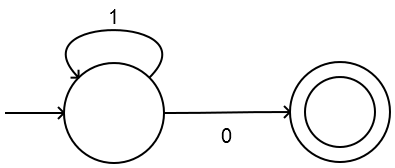
\includegraphics[scale=0.5]{DFAQ3.png}
    	\end{figure}

    \subsection{Language}
    
    	The language of balanced parenthesis is not regular.
    	To demonstrate it, let us consider a simplified version of the language
    	where we consider only a sequence of k left parenthesis followed by
    	a sequence of k right parenthesis, this simplified version forming
    	a subset of the language we wish to prove irregular :
    	\newline
    	$$\{(^k )^k\}$$

    	Using pumping lemmas, we can easily prove this language irregular by defining
    	$w = \{(^k )^k\}$. By the pumping lemma, there should be some decomposition
    	w = xyz with $|xy| \le p$ and $|y| \ge 1$ such that $x(y^i)z$
    	in L for every $i \ge 0$. \newline

    	Since $|xy| \le p$, we know that y can only contain a non-null sequence of
    	left parenthesis. This means that by pumping y and obtaining $xy^2 z$, we will
    	a sequence of parenthesis with more open parenthesis than closed parenthesis.
    	\newline

    	Thus, this sequence will never be part of our simplified language L, and since
    	this subset of the original language cannot be represent by a regular expression,
    	we can infer that the whole language similarly cannot be represented.
    	
    \section{Recursive descent}
    \subsection{Changes to the grammar}
    
    	The current grammar is by no means LL(1) as it is subject to both direct and
    	indirect recursion. The grammar must thus be changed as follow to become LL(1) :
    	\newline
    	
    	% En cas de besoin : http://smlweb.cpsc.ucalgary.ca/start.html
    	\begin{flushleft}
    	E -> T $E_1$ \\
    	$E_1$ -> and T $E_1$ | nand T $E_1$ | $\epsilon$ \\
    	T -> F $T_1$ \\
		T1 -> or F $T_1$ | nor F $T_1$ | epsilon \\
		F -> ( E ) | !F | id \\
		id -> true | false \\
		\end{flushleft}

    	This new grammar created using the rules specified in the slides describes
    	the same language but allows a LL parser to be made.

\end{document}
